\documentclass[12pt]{article}
\usepackage{amsmath, amssymb, graphicx, booktabs, geometry, hyperref}
\geometry{margin=1in}
\title{Project 2 (Report): Experimental Analysis of Bin Packing Algorithms}
\author{Aditya Singh}
\date{\today}

\begin{document}

\maketitle

\section{Introduction}
Bin packing is a classic combinatorial optimization problem with many practical applications. The objective is to pack a list of items, each with a size between 0 and 1, into the minimum number of bins of unit capacity. In this project, we experimentally evaluate the performance of five well-known bin packing algorithms:
\begin{itemize}
    \item Next Fit (NF)
    \item First Fit (FF)
    \item Best Fit (BF)
    \item First Fit Decreasing (FFD)
    \item Best Fit Decreasing (BFD)
\end{itemize}

The main metric of interest is the \emph{waste} $W(A)$ of an algorithm $A$ on a list of items, defined as the number of bins used minus the total size of all items. We estimate $W(A)$ as a function of the number of items $n$ by running each algorithm on random instances and analyzing the results.

\section{Algorithm Descriptions}
\begin{description}
    \item[Next Fit (NF):] Place each item in the current bin if it fits; otherwise, start a new bin.
    \item[First Fit (FF):] Place each item in the first bin (in order of creation) where it fits; open a new bin if necessary.
    \item[Best Fit (BF):] Place each item in the bin with the least remaining space where it fits; open a new bin if necessary.
    \item[First Fit Decreasing (FFD):] Sort items in decreasing order, then apply First Fit.
    \item[Best Fit Decreasing (BFD):] Sort items in decreasing order, then apply Best Fit.
\end{description}

\section{Experimental Setup}
\begin{itemize}
    \item For each $n \in \{10, 100, 500, 1000, 2500, 5000, 10000\}$, generate 20 random lists of $n$ items, each item uniformly in $[0, 0.35]$.
    \item Run each algorithm on each list.
    \item Record the number of bins used, total size, and compute the waste $W(A)$.
    \item Compute the average waste for each algorithm and $n$.
    \item Plot $W(A)$ vs $n$ on a log-log scale and fit a line to estimate the slope.
\end{itemize}

\section{Results}

\subsection{Waste Plots and Slope Estimates}
For each algorithm, the following plots show the average waste as a function of $n$ on a log-log scale, along with the estimated slope and waste function.

\begin{figure}[h!]
    \centering
    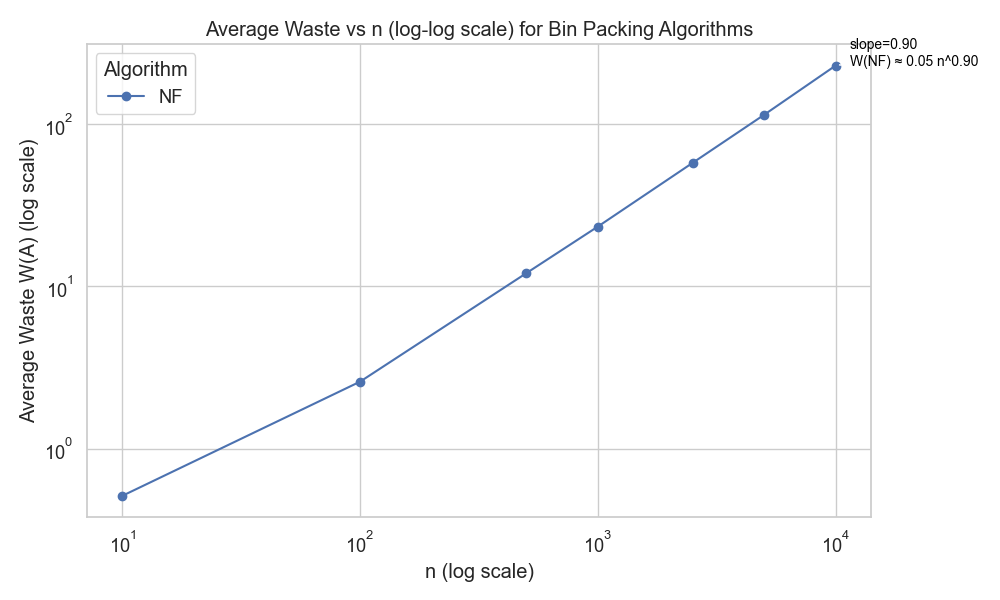
\includegraphics[width=0.8\textwidth]{waste_loglog_NF.png}
    \caption{Next Fit (NF): $W(\text{NF}) \approx 0.05 n^{0.90}$}
\end{figure}

\begin{figure}[h!]
    \centering
    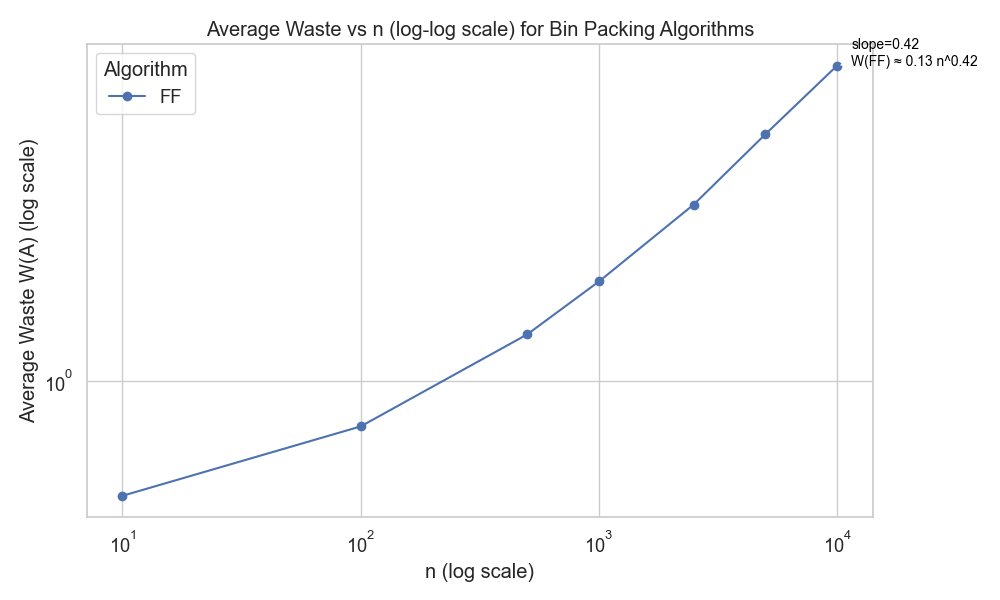
\includegraphics[width=0.8\textwidth]{waste_loglog_FF.png}
    \caption{First Fit (FF): $W(\text{FF}) \approx 0.13 n^{0.42}$}
\end{figure}

\begin{figure}[h!]
    \centering
    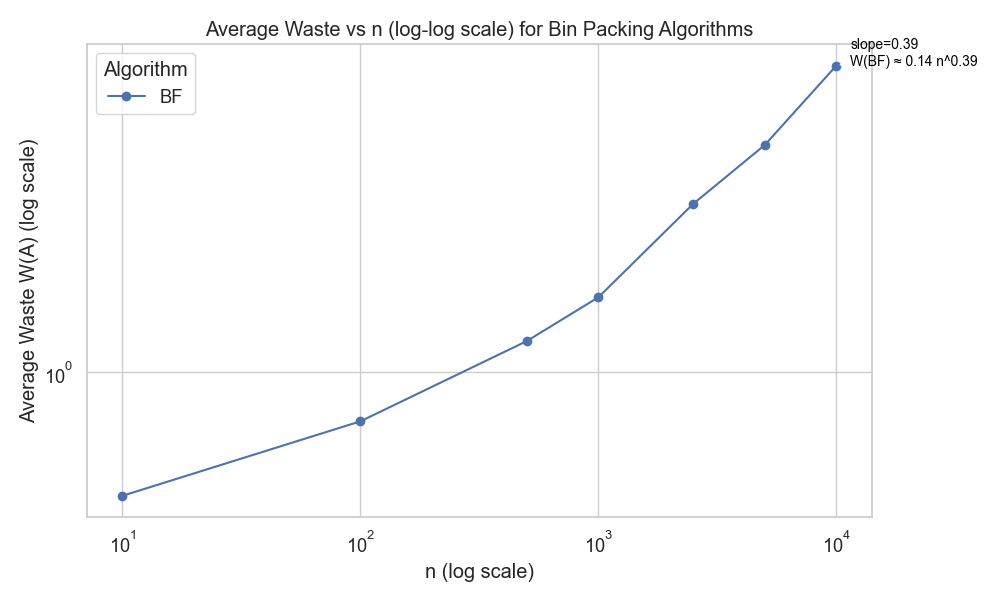
\includegraphics[width=0.8\textwidth]{waste_loglog_BF.png}
    \caption{Best Fit (BF): $W(\text{BF}) \approx 0.14 n^{0.39}$}
\end{figure}

\begin{figure}[h!]
    \centering
    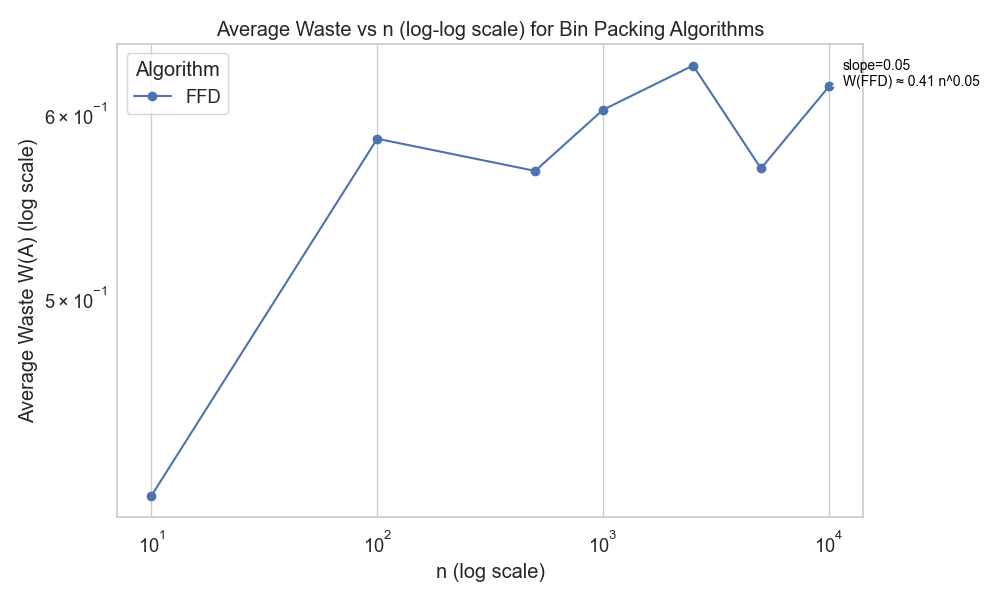
\includegraphics[width=0.8\textwidth]{waste_loglog_FFD.png}
    \caption{First Fit Decreasing (FFD): $W(\text{FFD}) \approx 0.41 n^{0.05}$}
\end{figure}

\begin{figure}[h!]
    \centering
    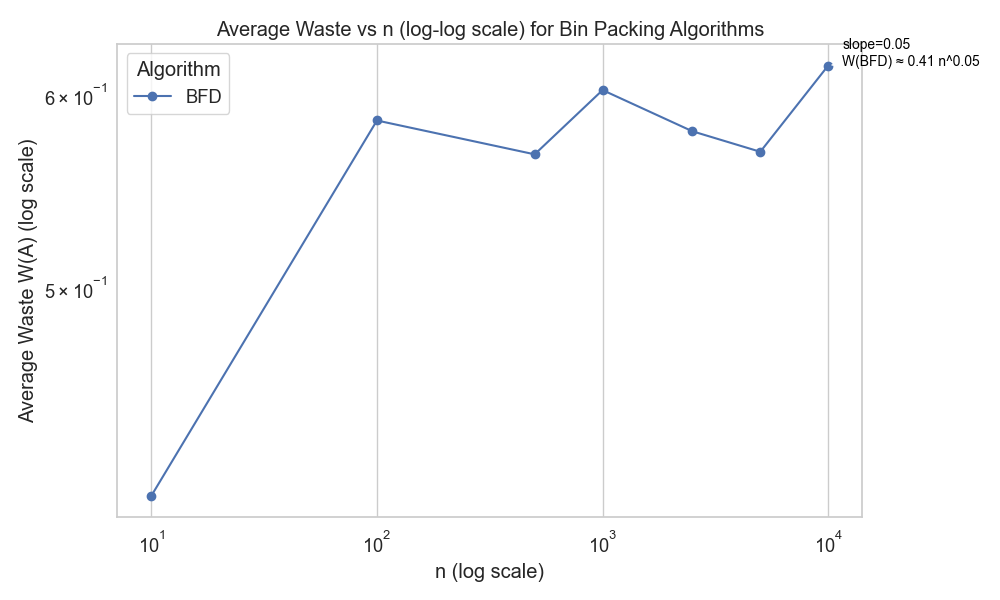
\includegraphics[width=0.8\textwidth]{waste_loglog_BFD.png}
    \caption{Best Fit Decreasing (BFD): $W(\text{BFD}) \approx 0.41 n^{0.05}$}
\end{figure}

\clearpage

\subsection{Summary Table}
\begin{table}[h!]
    \centering
    \begin{tabular}{lccc}
        \toprule
        Algorithm & Slope & Waste Function & Performance as $n$ Grows \\
        \midrule
        NF  & 0.90 & $0.05 n^{0.90}$ & Poor (waste grows quickly) \\
        FF  & 0.42 & $0.13 n^{0.42}$ & Moderate \\
        BF  & 0.39 & $0.14 n^{0.39}$ & Moderate \\
        FFD & 0.05 & $0.41 n^{0.05}$ & Excellent (almost constant) \\
        BFD & 0.05 & $0.41 n^{0.05}$ & Excellent (almost constant) \\
        \bottomrule
    \end{tabular}
    \caption{Summary of slopes and waste functions for each algorithm.}
\end{table}

\section{Analysis and Discussion}

The slope of the log-log plot indicates how quickly the waste grows as $n$ increases. Lower slopes are better. The results show:
\begin{itemize}
    \item \textbf{FFD} and \textbf{BFD} have the lowest slopes ($\approx 0.05$), meaning their waste grows extremely slowly with $n$.
    \item \textbf{NF} has the highest slope ($\approx 0.90$), so its waste increases rapidly as $n$ increases.
    \item \textbf{FF} and \textbf{BF} are intermediate, with moderate slopes ($\approx 0.39$--$0.42$).
\end{itemize}

\textbf{Why do FFD and BFD perform best?} Both algorithms sort the items in decreasing order before packing, allowing them to fill bins more efficiently and reduce the chance of leaving large gaps. This results in bins being packed more tightly and overall waste being minimized. The experimental results confirm this: both FFD and BFD have a very low slope, indicating that the waste grows almost negligibly as the number of items increases. In contrast, algorithms that do not sort the items (NF, FF, BF) leave more waste, especially as $n$ increases.

\section{Conclusion}

Our experiments show that \textbf{First Fit Decreasing (FFD)} and \textbf{Best Fit Decreasing (BFD)} are the best algorithms for minimizing waste in the bin packing problem, especially as the number of items grows. Their waste grows extremely slowly with $n$, making them the preferred choice for large-scale applications. For practical purposes, we recommend using FFD or BFD when minimizing waste is critical.

\end{document} 